\documentclass[a4paper,11pt]{article}
\usepackage[utf8]{inputenc}
\usepackage{algorithmic}
\usepackage{algorithm}
\usepackage{pst-plot}
\usepackage{graphicx}
\usepackage{endnotes}
\usepackage{graphics}
\usepackage{floatflt}
\usepackage{wrapfig}
\usepackage{amsfonts}
\usepackage{amsmath}
\usepackage{verbatim}
\usepackage{hyperref}
\usepackage{multirow}
\usepackage{pdflscape}
\usepackage{enumitem}
\usepackage[normalem]{ulem}

\usepackage{hyperref}
\hypersetup{pdfborder={0 0 0 0}}

\pdfpagewidth 210mm
\pdfpageheight 297mm 
\setlength\topmargin{0mm}
\setlength\headheight{0mm}
\setlength\headsep{0mm}
\setlength\textheight{250mm}	
\setlength\textwidth{159.2mm}
\setlength\oddsidemargin{0mm}
\setlength\evensidemargin{0mm}
\setlength\parindent{7mm}
\setlength\parskip{0mm}

\newenvironment{exercise}[1]{\paragraph{#1}\ \\}{
\medskip}
\newcommand{\question}[2]{\setlength\parindent{0mm}\ \\$\mathbf{Q_#1:}$ #2\ \\}

\author{\large{Tambet Matiisen, Raul Vicente, Zurab Bzhalava}}
\title{\huge{3rd Baltic-Nordic Summer School on Neuroinformatics (BNNI 2015)}\\\LARGE{Practice on Artificial Neural Networks}}

\begin{document}
\maketitle

%
% Intro
%
The 2014 Nobel prize in Physiology was awarded to Dr. John M. O'Keefe, Dr. May-Britt Moser and Dr. Edvard I. Moser for discovering particular cells in the brain that provide the sense of place and navigation. In this practice session, we are going to use computational approach to study the animal "GPS" system. In particular, we are going to use artificial neural networks to predict a rat's position based just on its hippocampal neural activity.

At first we divide the experimental arena into 16 blocks and approach this as a classification problem. Next we make the task harder by trying to predict the rat's position (X and Y coordinates) directly, i.e. address this as a regression problem. Finally we automate the tedious task of hyperparameter optimization using Whetlab. 

The data we use is multi-neuron electrophysiological recordings from the Buzsaki lab in New York. The data has been preprocessed as number of spikes in 500ms time window.

%
% Installation
%
\section{Technicalities}

You can use either Matlab or Octave to do the practice exercises. Matlab is faster and more user-friendly, but Octave is free and has been catching up with Matlab lately. Be sure to install at least version 3.8 of Octave, which includes the experimental GUI.
\begin{itemize}
	\item \textbf{Ubuntu:} \texttt{sudo apt-get install octave}. To start the GUI run this from command line: \texttt{octave --force-gui}. Then you can lock the application to the launch bar. 
	\item \textbf{Windows:} the most current version can be downloaded from here:\\ \url{https://ftp.gnu.org/gnu/octave/windows/}.
\end{itemize}

For Octave you will also need to install packages \texttt{statistics} and \texttt{nan}, which include some basic machine learning tools we use for calculating baseline performance. 

\begin{itemize}
	\item \textbf{Ubuntu:} \texttt{sudo apt-get install octave-statistics octave-nan}
	\item \textbf{Windows:} run this from Octave command line: \texttt{pkg install -auto -forge statistics}. Unfortunately the latest \texttt{nan} package does not compile under Windows, so you have to download version 2.7.1 manually from here: \url{http://sourceforge.net/projects/octave/files/Octave%20Forge%20Packages/Individual%20Package%20Releases/}, and install it from Octave command line with \texttt{pkg install -auto nan-2.7.1.tar.gz}.
\end{itemize}

If you are new to Matlab/Octave, then these are excellent tutorials to start with:
\begin{itemize}
	\item \url{https://en.wikibooks.org/wiki/Octave_Programming_Tutorial}
	\item \url{https://www.youtube.com/playlist?list=PLZ-E1VZLTeHMtUopmGx99KS775aHYP3e4}
\end{itemize}

Finally, for artificial neural networks we are going to use DeepLearnToolbox by Rasmus Berg Palm, which can be found from here: \url{https://github.com/rasmusbergpalm/DeepLearnToolbox}. It is also included with the tasks, so don't bother downloading it.

%
% ANN
%
\section{Artificial Neural Networks}

Tuning artificial neural networks can be frustrating experience. Many people have tried and given up before they start to get any useful results. In this practice session we hope to give you step-by-step guidelines on how to tune the learning parameters of neural network and how to squeeze out maximum performance from them. But beforehand we would like you to have a basic understanding how artificial neural networks work.

An artificial neural network consists of interconnected nodes, often called "neurons". Some of those nodes are input nodes -- they receive information from the outside world. Some of them are output nodes -- they provide the results of the calculation. Finally there are hidden nodes, which are just intermediate steps of computation.

\begin{figure}[h]
	\centering
	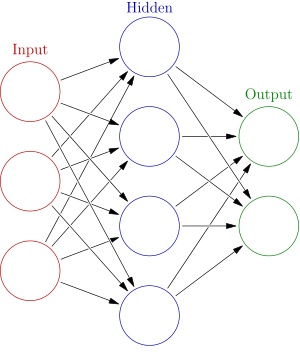
\includegraphics[width=0.25\textwidth]{ann.png}
	\caption{Artificial neural network with one hidden layer.}
\end{figure}

Nodes of artificial neural network are organized into layers. There are no connections between nodes in the same layer, only between layers -- input layer nodes are connected to first hidden layer nodes, first hidden layer nodes are connected to the second hidden layer nodes and so on until last hidden layer nodes are connected to the output layer. In simplest neural networks, called feed-forward neural networks, the connections are in one direction only -- from input towards output.

While artificial neurons are inspired by their biological counterparts, they are just cartoonish simplifications of actual neurons. Typical artificial neuron just multiplies its inputs with respective weights, sums the results and applies an activation function. 

\begin{figure}[h]
	\centering
	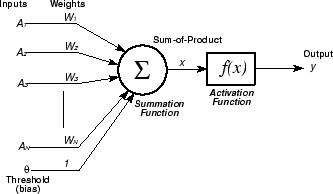
\includegraphics[width=0.55\textwidth]{neuron.png}
	\caption{Artificial neuron.}
\end{figure}

Common activation functions are $sigmoid(x)=\frac{1}{1 - e^{-x}}$ (squashes any real value to between $0$ and $1$), $tanh(x)=\frac{sinh(x)}{cosh(x)}$ (squashes any real value to between $-1$ and $1$) and $ReLU$ (rectified linear unit, $f(x)=max(x, 0)$). The purpose of activation functions is to add non-linearity into the calculations.

\begin{figure}[h]
	\centering
	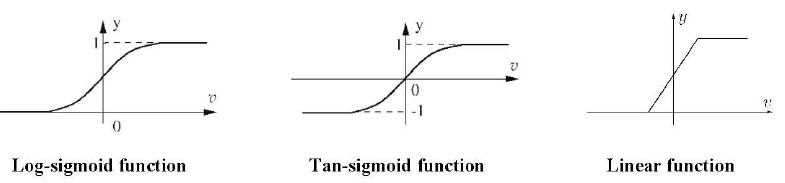
\includegraphics[width=0.8\textwidth]{activation_functions.png}
	\caption{Common activation functions.}
\end{figure}

\newpage

The beauty of artificial neural networks is, that they can learn to map inputs to outputs, given enough examples. The learning is accomplished by changing weights between neurons. The universal approximation theorem states, that any function can be approximated to a given precision using artificial neural network with just one hidden layer. In practice this result is irrelevant, because the claim that function can be represented by network does not say anything if this representation can be learned by the network. Still it is important to remember that artificial neural networks are nothing more than universal function approximators.

We start first by defining a loss function, which measures how good the networks' current prediction is -- how well its outputs match the expected values. Small loss is good, big loss is bad. The most common loss function is mean squared error (MSE) -- you just square all differences between predicted and expected values, sum over all output nodes and average over the training batch. It is easy to see, that better predictions result in lower loss values with MSE. If outputs of your network are probabilities, then you would use a different loss function (cross-entropy loss), but the general idea stays the same.

To learn we would need to change the weights in a way, that decreases the loss function. The most common method to achieve that is called gradient descent. First we take partial derivatives of the loss function with respect to each weight. These derivatives -- the gradients -- give us an estimate of how much changing each particular weight would affect the loss function. To calculate those derivatives efficiently in an artificial neural network we use the backpropagation algorithm. This algorithm basically consists in applying the chain rule to find the derivatives of bottom layers from the derivatives of upper layers. Not wanting to go into details in here, let's just assume that somehow we know the gradients and thus how much we should add to or subtract from each weight to make the loss decrease.

\begin{figure}[h]
	\centering
	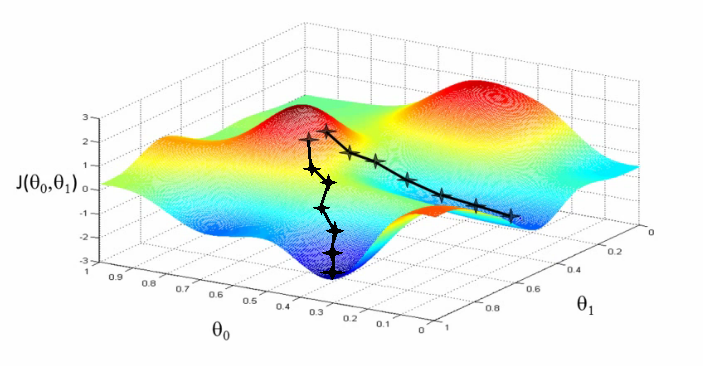
\includegraphics[width=0.8\textwidth]{gradient_descent.png}
	\caption{Gradient descent.}
	\label{gradient_descent}
%
% $J(\theta_1,\theta_2)$ is the loss function, $\theta_1$ and $\theta_2$ are the weights (suppose we have only two of them).
%
\end{figure}

The complex nature of artificial neural networks means, that there might be more than one set of weight values for which the loss function has the minimal value. Moreover there are many local minimas, making it a non-convex optimization problem. Often the metaphore of "loss landscape" is used -- if you plotted loss value over many weight value combinations, then it would form a landscape of many hills and valleys. If you just followed the gradient (go downhill in the direction of the steepest descent), then it is easy to get stuck in a local minima (a shallow valley). People have come up with many techniques to work around this issue, but in principle it remains unresolved. Good news is that many of the local minimas are good enough and that there are plenty of them.

\section{Preprocessing}

TBD

\newpage

%
% Classification
%
\section{Classification}

In this exercise we divide the arena into 16 regions and try to predict the region where the rat is currently located in from the activity of 61 neurons in the hippocampal area of the brain.\\

Start by running the code in \texttt{classification.m} and observing the results:

\begin{enumerate}
	\item First you should see the baseline performance of a linear classifier. This part of the code is added just to remind you, that artificial networks are heavy artillery and should be used only if simpler methods do not give satisfactory results. 
	\item Thereafter you will be shown the training progress of the artificial neural network. You can ignore the command-line output and concentrate on the two figures shown during training:
	\begin{itemize}
		\item The first one displays the loss function value for both training and validation set. As this is a classification task we are using cross-entropy loss function. Its value is actually rather meaningless, we are more interested in the dynamics -- does it decrease, how fast, is the learning stable?
		\item The second figure shows the misclassification rate -- the fraction of training samples for which the predicted class was wrong. You can calculate accuracy by subtracting this number from 1. Again, error rates for both the training and validation set are shown.
	\end{itemize}
	Usually those two graphs are correlated, so it suffices to only pay attention to the latter. Also the validation set performance is more important than the training set performance.
	\item After training is completed you should see the accuracy of neural network printed out. At first it might not be much better than the linear classifier.
	\item Finally the confusion matrix is shown. Confusion matrix summarizes the errors our classifier made -- which classes were mistaken for which other classes.
\end{enumerate}

\textbf{Your job is to tune this neural network to have an accuracy of at least 70\%.}\\

\begin{figure}[h]
	\centering
	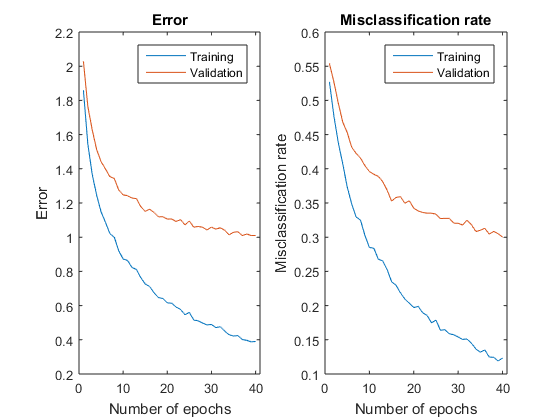
\includegraphics[width=0.66\textwidth]{training_loss.png}
	\caption{Example of network achieving 70\% accuracy.}
\end{figure}

\begin{enumerate}
	\item First you should start by finding the optimal \textbf{learning rate}. Learning rate is the one most important learning parameter, it determines the step size on loss landscape. 
	\begin{itemize}	
		\item Too big learning rate -- you step over valleys and never go deep into them. 
		\item Too small learning rate -- you end up in the closest valley however shallow it might be. 
	\end{itemize}
	Usually you try learning rate values in decreasing powers of 10, i.e. 1, 0.1, 0.01, 0.001 and so on. Repeat this until graphs are stable and the validation accuracy does not improve any more. Basically you want to use the highest learning rate, that does not blow up your loss.
	\item Thereafter you might want to increase the \textbf{number of hidden nodes} to see if validation accuracy improves. More hidden nodes means the network can learn to approximate increasingly complicated functions. Traditionally we use powers of 2 as the number of hidden nodes, i.e. use twice as much hidden nodes as previously.
	\item After that you should use \textbf{momentum} to speed up learning. Momentum adds inertia to weight updates -- at each update we do not just go towards the gradient, but also take in consideration the previous weight update. This results in a faster movement on long descents in one direction. Sometimes momentum may overshoot resulting in zig-zags on the graphs, but usually it helps to reach to minima faster. Usual values to try are 0.5, 0.9 and 0.95.
	\item By now you should observe massive overfitting -- training set error is much smaller than validation set error. Basically network memorizes the training set and does not generalize to the validation set. There are several ways how to deal with overfitting:
	\begin{description}
		\item[Get more training data.] Data is the most effective regularizer, so if possible you should always use that option. However, in the reality it is rarely easy to get additional data. In such cases the following methods come to your aid.
		\item[Use weight decay.] This is a well-known technique, that forces weights to have small values. It is implemented by adding a regularization term to the loss function, which results in decreasing all weights by some fraction of their current value during each training iteration (hence "weight decay"). You should start with low values of $10^{-4}$ and go up in powers of 10 until validation set accuracy does not improve any more.
		\item[Use dropout.] Dropout disables a random subset of hidden nodes during each training step. This forces nodes to be more individualistic, because they are not able to count on the other nodes being present. During testing all nodes are enabled, but their activation values must be decreased in order produce on average the same amount of input to the subsequent layer. This functions also as a crude approximation to the ensemble method -- basically we are averaging the behaviour of many networks with shared weights. Common dropout fraction to use is 0.5, but in some cases lower values might work better.

\begin{figure}[h]
	\centering
	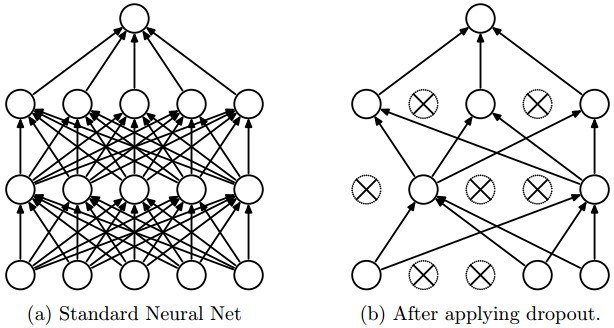
\includegraphics[width=0.6\textwidth]{dropout.jpg}
	\caption{Dropout.}
\end{figure}

	\end{description}

	Finally, some amount of overfitting is inevitable and healthy with neural networks. So as long as validation set accuracy improves, do not worry too much about it.

	\item Once you think your learning parameters are good enough, you should try to learn longer -- increase the \textbf{number of epochs}. One epoch is a full training session over the entire training set. Usually the loss function plateaus at some point and there is no point in training any further. You should figure out where this point is by trying say 100 epochs. To save time in further finetuning we advise you to limit the number of epochs to when the plateau was reached.

	\item As gradient descent explores the loss landscape, there might be gradually more fine-grained valleys to descend to. With initial learning rate you may just step over those valleys or step out of them once you are in. For that reason it is usually a good idea to decrease the learning rate once the loss function has plateaued. Most commonly we would do it in powers of 10, i.e. multiply learning rate by 0.1. However, instead of decreasing learning rate in big steps, the DeepLearnToolbox applies a scaling rate after each learning epoch. To achieve a multiplier of 0.1 after $n$ epochs you need to calculate the approximate per-epoch scaling rate by

$$
scaling\_learningRate = \sqrt[n]{0.1}
$$

\end{enumerate}

Mind that there is a delicate interplay between all the parameters -- if you increase the number of nodes, you might also need to lower the learning rate; if you increase the weight decay, you might need to also increase the learning rate; dropout usually works better with bigger number of nodes and so on. The rules of thumb given here do not guarantee you the best results, they just help you to quickly identify the ranges of parameters that work OK, but from that point onwards you are on your own.\\

For this task you should not invest too much effort into choosing:

\begin{itemize}
	\item \textbf{Batch size.} In stochastic gradient descent (SGD) you divide training set into batches of random samples and train one batch at a time. You use the average gradient of all samples in a batch to perform the weight update. If the batch size is too small (not representative of training set distribution), your gradient may not point towards what would be the best direction for the entire training set and the gradient descent will walk around aimlessly. If the batch size is too big, you always step to right direction, but each training iteration is just very time consuming. It is good to use the smallest batch size which is still sufficiently representative of the training set. But in practice batch size is often more restricted by the amount of memory your GPU has or how many parallel computations it can handle.
	\item \textbf{Activation function.} For small shallow networks use $tanh$. Modern deep networks use $ReLU$ to combat the vanishing gradient problem and to maximize performance. But this is not so much of an issue with small networks.
	\item \textbf{Depth of the network.} While hierarchical representation of features is the main selling point of artificial neural networks, the benefits of hierarchy show up only with more complex networks architectures like convolutional networks. These networks make use of the locality property of information. For small fully-connected networks usually one to three layers is enough.
 \end{itemize}

%
% Regression
%
\section{Regression}

In this exercise we try to predict the rat's location directly. This time we are going to use activity of all 70 neurons as input. Outputs of the network are the X and Y coordinates of the rat.\\

Start again by running the code in \texttt{regression.m} and observing the results:

\begin{enumerate}
	\item First you should see the baseline performance of linear regression. The result is given as an average Euclidian distance between predicted and actual rat location.
	\item Then you should observe the training progress of your artificial neural network. This time there is only one figure -- the loss. For regression we are using the classical mean square error loss (MSE). Again, you should pay more attention to validation set loss than training set loss.
	\item After that you should see the performance of neural network printed out. Again, at first it might not be much better than linear regression.
	\item Finally 20 pairs of predicted and actual locations are shown. You can tune the number of examples shown or duration of the pause between them.
\end{enumerate}

\textbf{Your job is to achieve as good average distance as you can!}\\

Use all the tricks you learned from the previous exercise. As the dataset is bigger this time, you might initially want to choose smaller subset of samples to work with. This way the training completes in minutes and you can iterate fast. Once you have successfully overfitted the smaller dataset, try full dataset and see if performance on validation set improves.

%
% Whetlab
%
\section{Whetlab}

As you probably saw with previous exercises, choosing the right hyperparameters can be tedious task. One of the methods that can help in this situation is Bayesian optimization. This is a specialized technique for finding the maximum values of functions that are very challenging to evaluate, due to their being very expensive or noisy. Hyperparameter optimization is one of such difficult problems -- training a machine learning system can be time and energy-consuming taking hours or even days. But the applications of Bayesian optimisation are not limited to machine learning -- you could use it to suggest new settings for lab experiments or for tuning marketing tactics. Whetlab is a startup by top machine learning experts, that makes using Bayesian optimization especially easy to use. Unfortunately it works only in Matlab.\\

 Start by going over the code in \texttt{whetlab\_regression.m}:

\begin{enumerate}
	\item First half should already be familiar from previous exercise.
	\item Thereafter the hyperparameters for Whetlab optimization are defined. \textbf{Your job is to fill in the ranges of those parameters based on the experience from previous exercises!} Notice how we use log scale for the learning rate and the number hidden nodes.
	\item After that a new experiment is created using \texttt{whetlab()} function. \textbf{Make sure you include your name in the experiment name!} For the first run, the resume option must be set to $false$, but for the next runs it must be $true$.
	\item Next, 10 experiments are run using hyperparameter values suggested by Whetlab. You can first run the commands in that loop manually and observe the results. \textbf{Can you guess what would be the first values Whetlab suggests?}
	\item Once you have made sure the code works as expected, you can run it for 10, 20 or 40 loops. While computer is crunching the numbers, you might want to read short introduction to Bayesian optimization from here: \url{https://www.whetlab.com/technology/}.
	\item Finally the code plots out two graphs of the results. Whetlab homepage includes many more useful visualizations, but for that you have to sign up for the closed beta yourself: \url{https://www.whetlab.com/beta-signup/}.
\end{enumerate}

That's all, hope you enjoyed it!

\end{document}
